%=================================================================
\section{Introduction}\label{sec-intro}
\subsection{Describe the Problem}
\smallskip
This is a problem with time-series prediction. Many information are given about daily sales data.The raw dataset contains train set with 2935849 samples and 214200 unlabeled samples as test set. Through the train data, predict total sales for every product and store in the next month..
\subsection{Interpret the Data}
\smallskip
Here's the data in the dataset.\\
\bigskip
\centerline{\normalsize{Table 1:Data}}
\begin{tabular}{cp{4cm}p{4cm}}
	\hline
	Name&Description&Attribute\\
	\hline
	sales\_train.csv& Training set(data from January 2013 to October 2015)&date,date_block_num, shop_id,item_id, item_price,item_cnt_day\\
	test.csv& Test set(Predict sale in November 2015) & ID,shop_id,item_id\\
	items.csv& Supplementary information of products &item_name, item_id, item_category_id\\
	shops.csv& Supplementary information of shops & shops_name,  shops_id\\
	item_categories.csv& Supplementary information of item categories & item_categories_name, item_categories_id\\
	sample_submission.csv& Format of submission & ID,item_cnt_month\\
	\hline
\end{tabular}
\subsection{Evaluation Criteria}
Before experiment, determine the evaluation methods to assess the model performance is very important, usually it has the RMSE methods to evaluate.
\section{Data Processing} \label{sec-preliminaries}	
\subsection{Missing Value and NaN Value} There are no missing value and none value.
	\begin{figure}[htb]
	\centering
	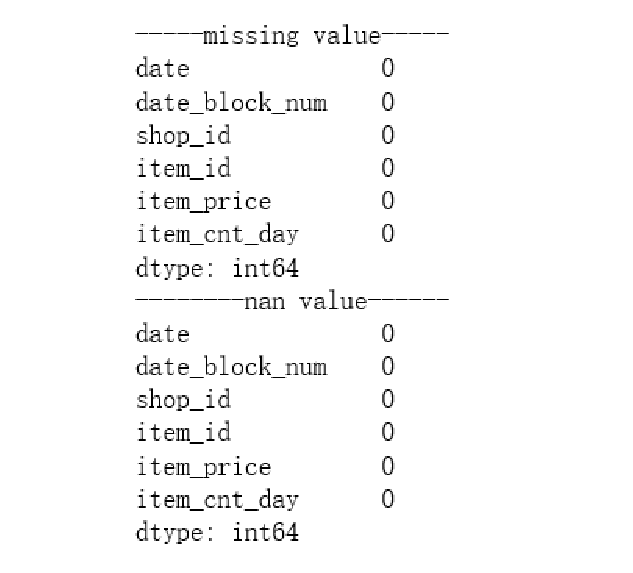
\includegraphics[width=8cm, height=6cm]{figures/miss.eps}\\
	\caption{Missing Value and NaN Value
	}\label{straddltimeScale}
\end{figure}
\subsection{Outliers and Duplicate Data} Filter duplicate data, outliers and data with price less than zero.
\begin{figure}[htb]
	\centering
	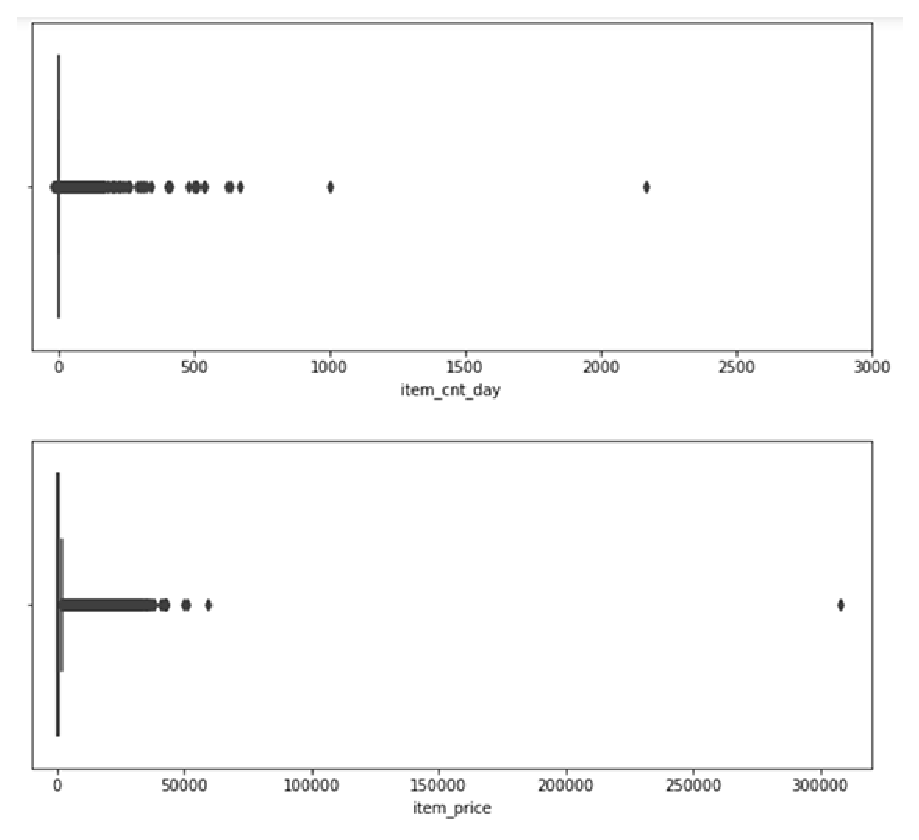
\includegraphics[width=10cm, height=8cm]{figures/outliers.eps}
	\caption{Outliers Data
	}\label{straddltimeScale}
\end{figure}

\subsection{Process Shops Set} Some shops have same shop name and different shop ID, such as ID of 39 and 40,10 and 11,0 and 57, 58 and 1. Then fliter the test set and modify the shop ID based on the test.
On the other hand, the report analyses shops name and finds the name can be divided into three parts: shop’s city,shop’s type and the shop’s name. Encoding shops information is able to reduce memory usage and find a connection with sales.

\subsection{Process Items Set} Some items have same item name and different item ID, such as ID of 2514 and 2558,2968 and 2970,5061 and 5063, 14537 and 14539,19465 and 19475,19579 and 19581
. Then fliter the test set and modify the item ID based on the test.

\subsection{Process Categories Set}  Analyses categories name and finds the name can be divided into two parts: category's type-category's subtype. Encoding shops information is able to reduce memory usage and find a connection with sales.

\subsection{Sales Analysis}	Figure3 shows that total sales every month are decreased over time. This reason probably is shops and items are decreased. By analyzing the data, there are many discontinued items in figure4 and these shops are closed:closed shops:0,1,8,11,13,17,23,27,29,30,32,33,40,43,51,54.
	\begin{figure}[htb]
	\centering
	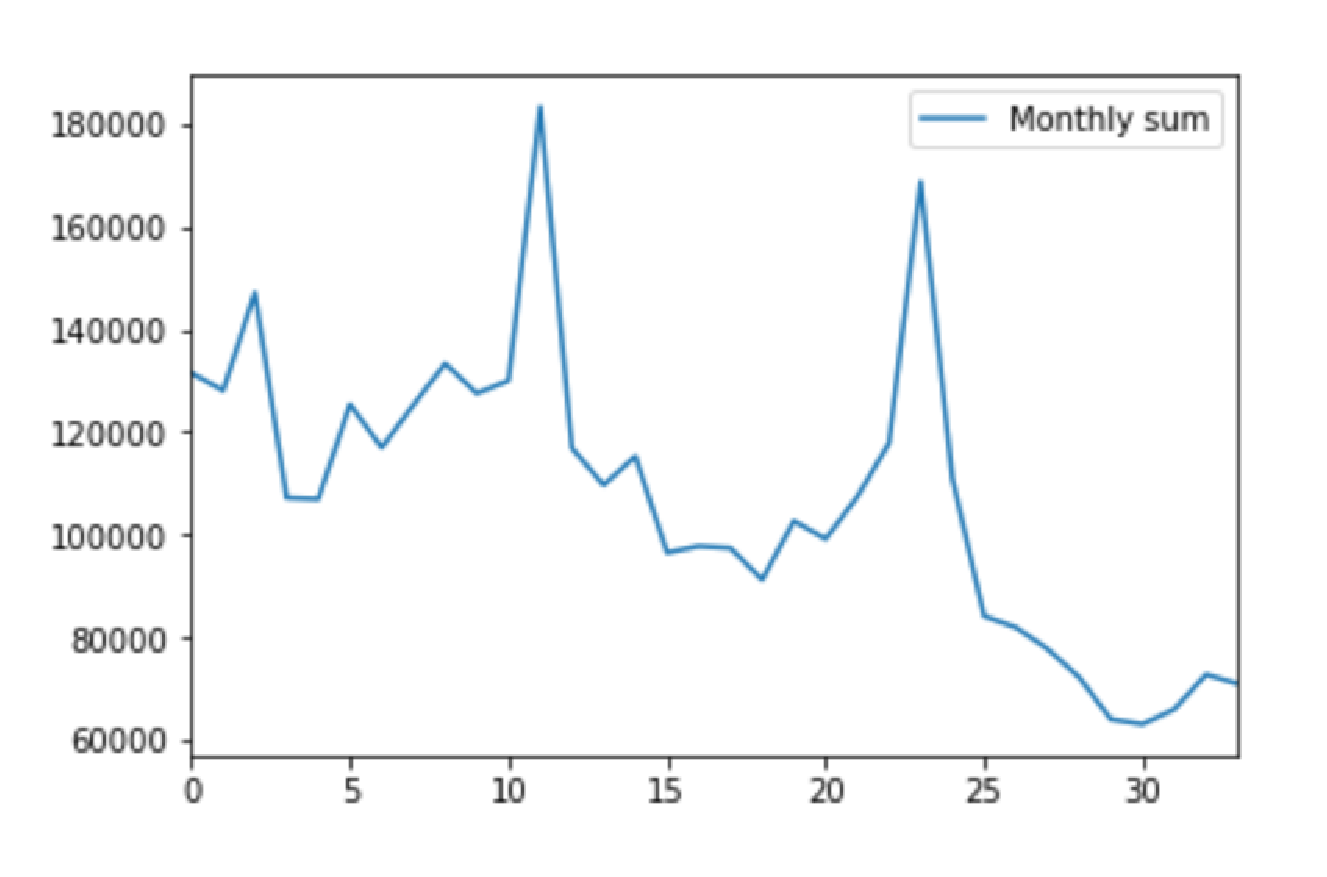
\includegraphics[width=10cm, height=6cm]{figures/sum.eps}
	\caption{Total Sales Over Time
	}\label{straddltimeScale}
\end{figure}
\begin{figure}[htb]
	\centering
	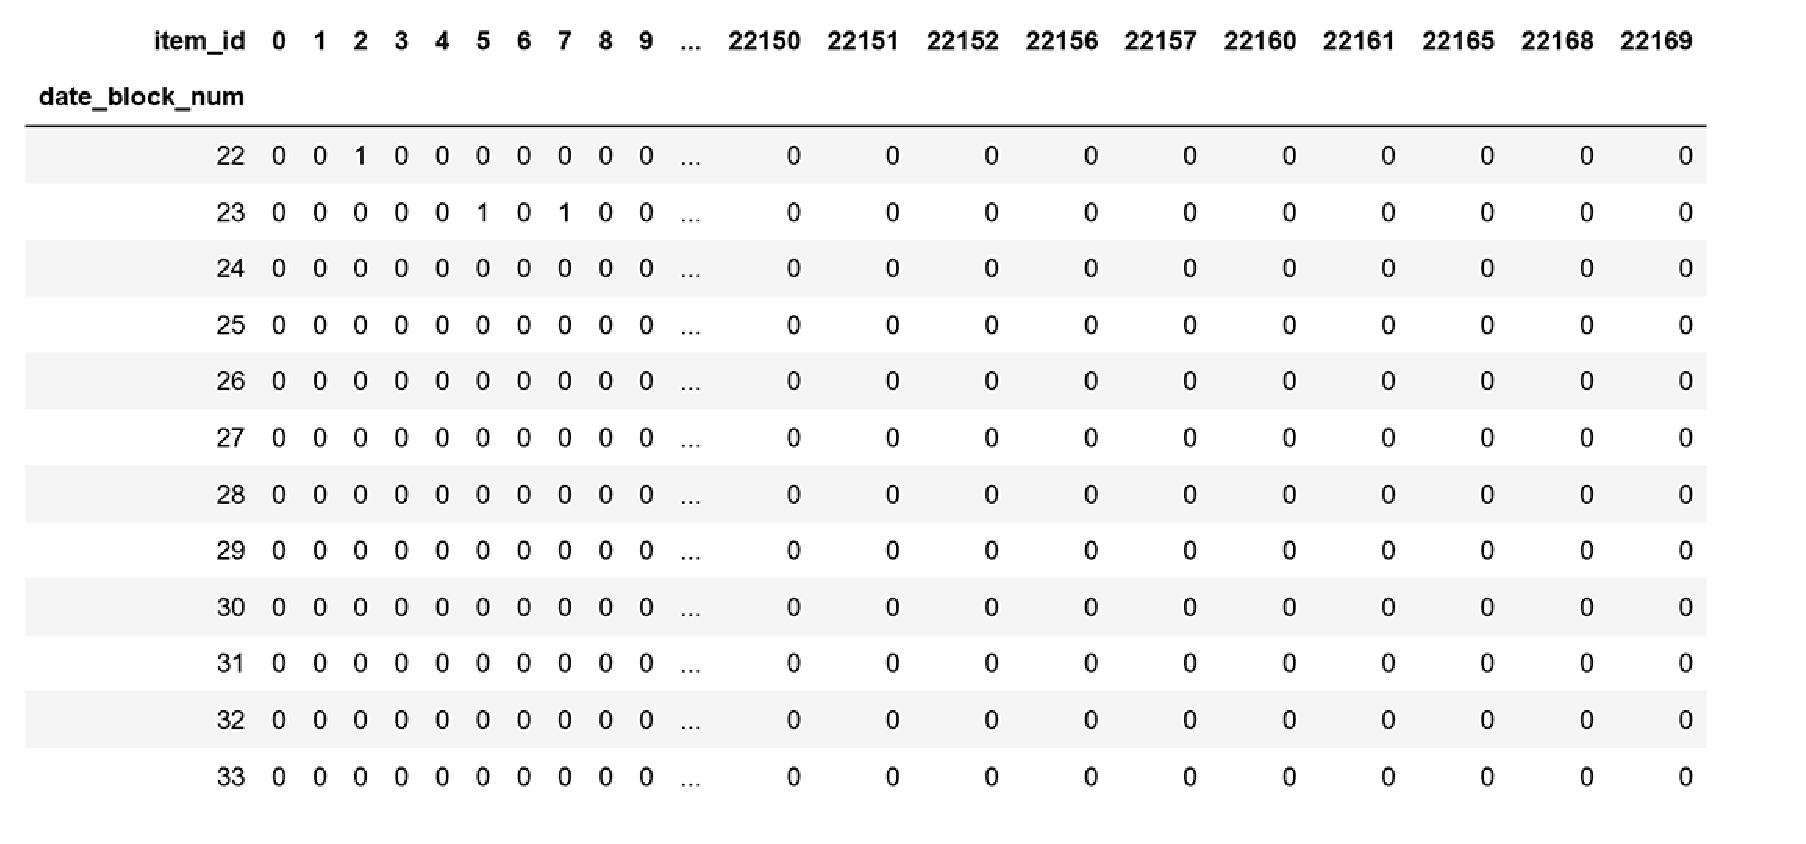
\includegraphics[width=12cm, height=6cm]{figures/stopitems.eps}
	\caption{Discontinued Products
	}\label{straddltimeScale}
\end{figure}
\section{Feature Selection} \label{sec-method}
\subsection{Data Feature}	
Data Feature mainly includes the features that analysing in the previous chapters, such as shop id and various codes. The specific features are shown below.
	\begin{figure}[htb]
	\centering
	\includegraphics[width=13cm, height=5cm]{figures/feature.eps}
	\caption{Data Feature
	}\label{straddltimeScale}
\end{figure}

\subsection{Monthly Sales Feature}	
\begin{itemize}
	\item average monthly sales of items 
	\item average monthly sales of shops 
	\item average monthly sales of categories
	\item average monthly sales of types and subtypes
	\item average monthly sales of shop's city-item
	\item average monthly sales of shop's type-item
\end{itemize}
\subsection{Historical Feature} From figure3 and materials searched in the Internet, historical month delays are set with 1,2,3,6 and 12, and the historical features are below. Finally, first 12 months records and NAN records should be deleted.
	\begin{itemize}
		\item monthly sales of items 
		\item average monthly sales of shops 
		\item average monthly sales of items
		\item average monthly sales of categories
		\item average monthly sales of types and subtypes
		\item average monthly sales of shop's city-item
		\item average monthly sales of shop's type-item
\end{itemize}
\section{Experiment and Analysis} \label{sec-experiment}
\noindent Using lightgbm to predict the sales. And in the final database, change zero to closed shops and discontinued items.\\
In the midterm report, XGBoost is used to predict the sales. And in the final report, Lightgbm is used to predict the sales. Because Lightgbm has the faster speed and higher accuracy than XGBoost.\\                                                         
XGBoost \cite{{BJL11J01}} is to establish K regression trees so that the predicted value of the tree group is as close as possible to the true value (accuracy) and has the greatest generalization ability. From a mathematical point of view, this is a functional optimization, multi-target.
Lightgbm\cite{{BJL11J02}} is a distributed gradient promotion framework based on decision tree algorithm. Lightgbm is designed to provide a data science tool with high efficiency, low memory consumption, high accuracy, supporting parallel and large-scale data processing
The final score is 1.04885 and get the middle rank.\\
Figure6 shows the feature importance of sales.\\
\begin{figure}[htb]
	\centering
	\includegraphics[width=13cm, height=5cm]{figures/light.eps}
	\caption{Feature Importance
	}\label{straddltimeScale}
\end{figure}
\noindent The result:
	\begin{itemize}
	\item score:0.93740
	\smallskip
	\item rank:3027/873
\end{itemize}

\section{Conclusions} \label{sec-conclusions}
\begin{itemize}
	\item  Exploratory data analysis and data processing is very important for the competition. Exploratory data analysis help to have a certain understanding of the overall appearance of the data, which will help later modeling and analysis. And data processing includes dealing with missing data and outliers, processing datasets and others.
	\item The most important thing is feature engineering. In the midterm report, several features are selected and some information in database is not used. And in this report, more features are selected, such as historical features and monthly sales feature. 
	\item	Compare to midterm presentation, RMSE decreased from 1.04885 to 0.93740. The reason mainly is more features and different modeling. In the figure of feature importance and monthly sales, some historical feature play an important role. And lightgbm model's and xgboost model's result have a marginal difference, but processing speed of lightgbm model is faster.
\end{itemize}

